\subsection{Masks, surplus cells and prime counts}
\label{sec:masks}

\begin{figure}[tbp]
  \centering
  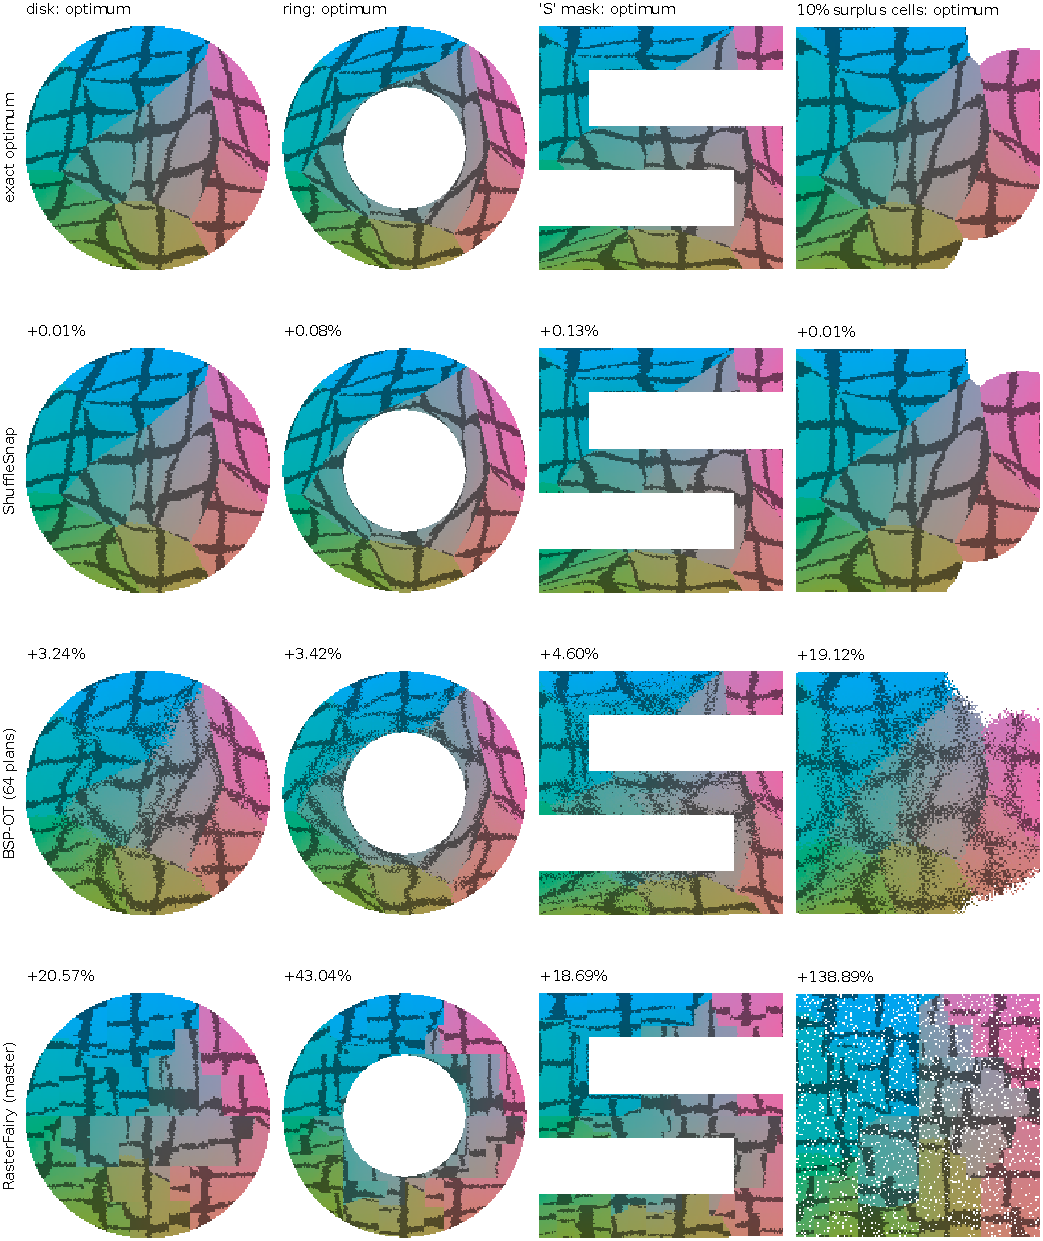
\includegraphics[width=\linewidth]{figures/fig_masks.pdf}
  \caption{A 20{,}000-point subset of the MNIST UMAP embedding on a disk, a ring, an
  S-shaped mask, and a rectangle with 10\% surplus cells (instance seed 1; colors encode
  input position as in Figure~\ref{fig:visual}; white = empty or masked). Numbers are
  excess over the certified optimum. With surplus cells, the optimum leaves one contiguous
  region empty, far from the data, and \ShuffleSnap-balanced finds the same region.
  BSP-OT's partial matching leaves ragged holes along the boundary, and RasterFairy
  removes surplus cells at random before slicing.}
  \label{fig:masks}
\end{figure}

\begin{table}[tbp]
\centering\scriptsize
\setlength{\tabcolsep}{3.5pt}
\caption{Excess over the certified optimum (\%) on non-square targets, $N=20{,}000$, mean of
instance seeds 1--3 (all 24 exact runs certified). ``Surplus ($<$1 row)'' is the full
$W\times H$ rectangle holding $N$ points, with fewer than $W$ empty cells;
``10\% surplus'' has $1.1N$ cells.}
\label{tab:masks}
\resizebox{\linewidth}{!}{\begin{tabular}{llrrrrrr}
\toprule
target & points & SS fast & BSP 16 & SS bal. & BSP 64 & SS qual. & RF master \\
\midrule
surplus ($<$1 row) & uniform & 6.31 & 90.3 & 3.10 & 85.0 & 1.37 & 56.6 \\
surplus ($<$1 row) & Gaussian mixture & 0.033 & 8.41 & 0.013 & 7.95 & 0.010 & 17.2 \\
surplus ($<$1 row) & spiral & 0.099 & 19.9 & 0.006 & 11.5 & 0.003 & 32.4 \\
surplus ($<$1 row) & MNIST UMAP & 0.082 & 16.5 & 0.020 & 5.29 & 0.011 & 43.6 \\
\addlinespace
10\% surplus & uniform & 3.81 & 108.9 & 0.91 & 58.7 & 0.25 & 350.5 \\
10\% surplus & Gaussian mixture & 0.43 & 30.5 & 0.055 & 17.6 & 0.012 & 71.6 \\
10\% surplus & spiral & 0.61 & 26.2 & 0.071 & 19.3 & 0.012 & 157.9 \\
10\% surplus & MNIST UMAP & 0.077 & 29.4 & 0.007 & 22.8 & 0.003 & 146.2 \\
\addlinespace
4:1 rectangle & uniform & 2.64 & 32.3 & 1.34 & 23.9 & 0.45 & 26.4 \\
4:1 rectangle & Gaussian mixture & 0.23 & 1.44 & 0.024 & 0.81 & 0.004 & 6.70 \\
4:1 rectangle & spiral & 0.34 & 4.33 & 0.067 & 2.34 & 0.022 & 15.4 \\
4:1 rectangle & MNIST UMAP & 0.18 & 2.07 & 0.014 & 1.28 & 0.003 & 11.6 \\
\addlinespace
disk & uniform & 0.034 & 8.64 & 0.014 & 6.74 & 0.006 & 11.4 \\
disk & Gaussian mixture & 0.016 & 5.43 & 0.003 & 4.27 & $<$0.001 & 37.0 \\
disk & spiral & 0.024 & 5.19 & 0.007 & 2.48 & 0.003 & 23.6 \\
disk & MNIST UMAP & 0.022 & 4.49 & 0.006 & 2.77 & 0.002 & 20.3 \\
\addlinespace
ring & uniform & 0.067 & 9.28 & 0.028 & 6.73 & 0.006 & 53.6 \\
ring & Gaussian mixture & 0.11 & 6.75 & 0.048 & 4.81 & 0.018 & 35.9 \\
ring & spiral & 0.048 & 7.73 & 0.014 & 3.83 & 0.016 & 47.9 \\
ring & MNIST UMAP & 0.14 & 4.77 & 0.070 & 3.11 & 0.025 & 43.2 \\
\addlinespace
S mask & uniform & 16.6 & 12.1 & 1.43 & 9.30 & 0.88 & 60.8 \\
S mask & Gaussian mixture & 0.63 & 4.11 & 0.057 & 2.99 & 0.036 & 32.4 \\
S mask & spiral & 3.27 & 12.5 & 0.26 & 4.79 & 0.19 & 56.8 \\
S mask & MNIST UMAP & 1.55 & 6.23 & 0.12 & 4.53 & 0.093 & 19.0 \\
\bottomrule
\end{tabular}
}
\end{table}

Table~\ref{tab:masks} and Figure~\ref{fig:masks} cover non-square targets.
\begin{itemize}
\item \textbf{Convex masks.} On disks and rings, every \ShuffleSnap\ preset stays within
  0.25\% (baseline) and 0.07\% (balanced) of the optimum. BSP-OT is at 2.5--9\% and
  RasterFairy at 11--54\%.
\item \textbf{The S-shaped mask.} This is the baseline's worst case. With uniform points
  it is 18.3\% above optimal, worse than BSP-OT with 64 plans (13.2\%); with the spiral it
  is 7.3\%. The mechanism is the one in Figure~\ref{fig:failures}: coarse strides route
  mass across the bays. The $\sqrt2$ schedule repairs most of this. Balanced reaches
  1.3\% and 0.26\%, and quality 0.13\% and 0.04\%.
\item \textbf{Surplus cells.} When the solver must also choose the empty cells, the baseline
  degrades noticeably: 0.7--4.4\% with 10\% surplus, and 8.4\% for uniform points with
  less than one row of surplus. Balanced stays below 1\% everywhere except that last
  case (3.1\%), and quality stays below 1.4\%. Surplus is where the comparators suffer
  most. With 10\% surplus, BSP-OT's partial matching is 18--109\% above optimal, and
  RasterFairy, which picks the empty cells at random, is 72--350\% above optimal. With
  less than one row of surplus, they are at 5--90\% and 17--57\%.
\end{itemize}
